\section{Architektur}
\label{sec:Architektur}

\subsection{Rahmenbedingungen}
\begin{figure}[H]
    \begin{center}
    		% GFX Trim left bottom right top
        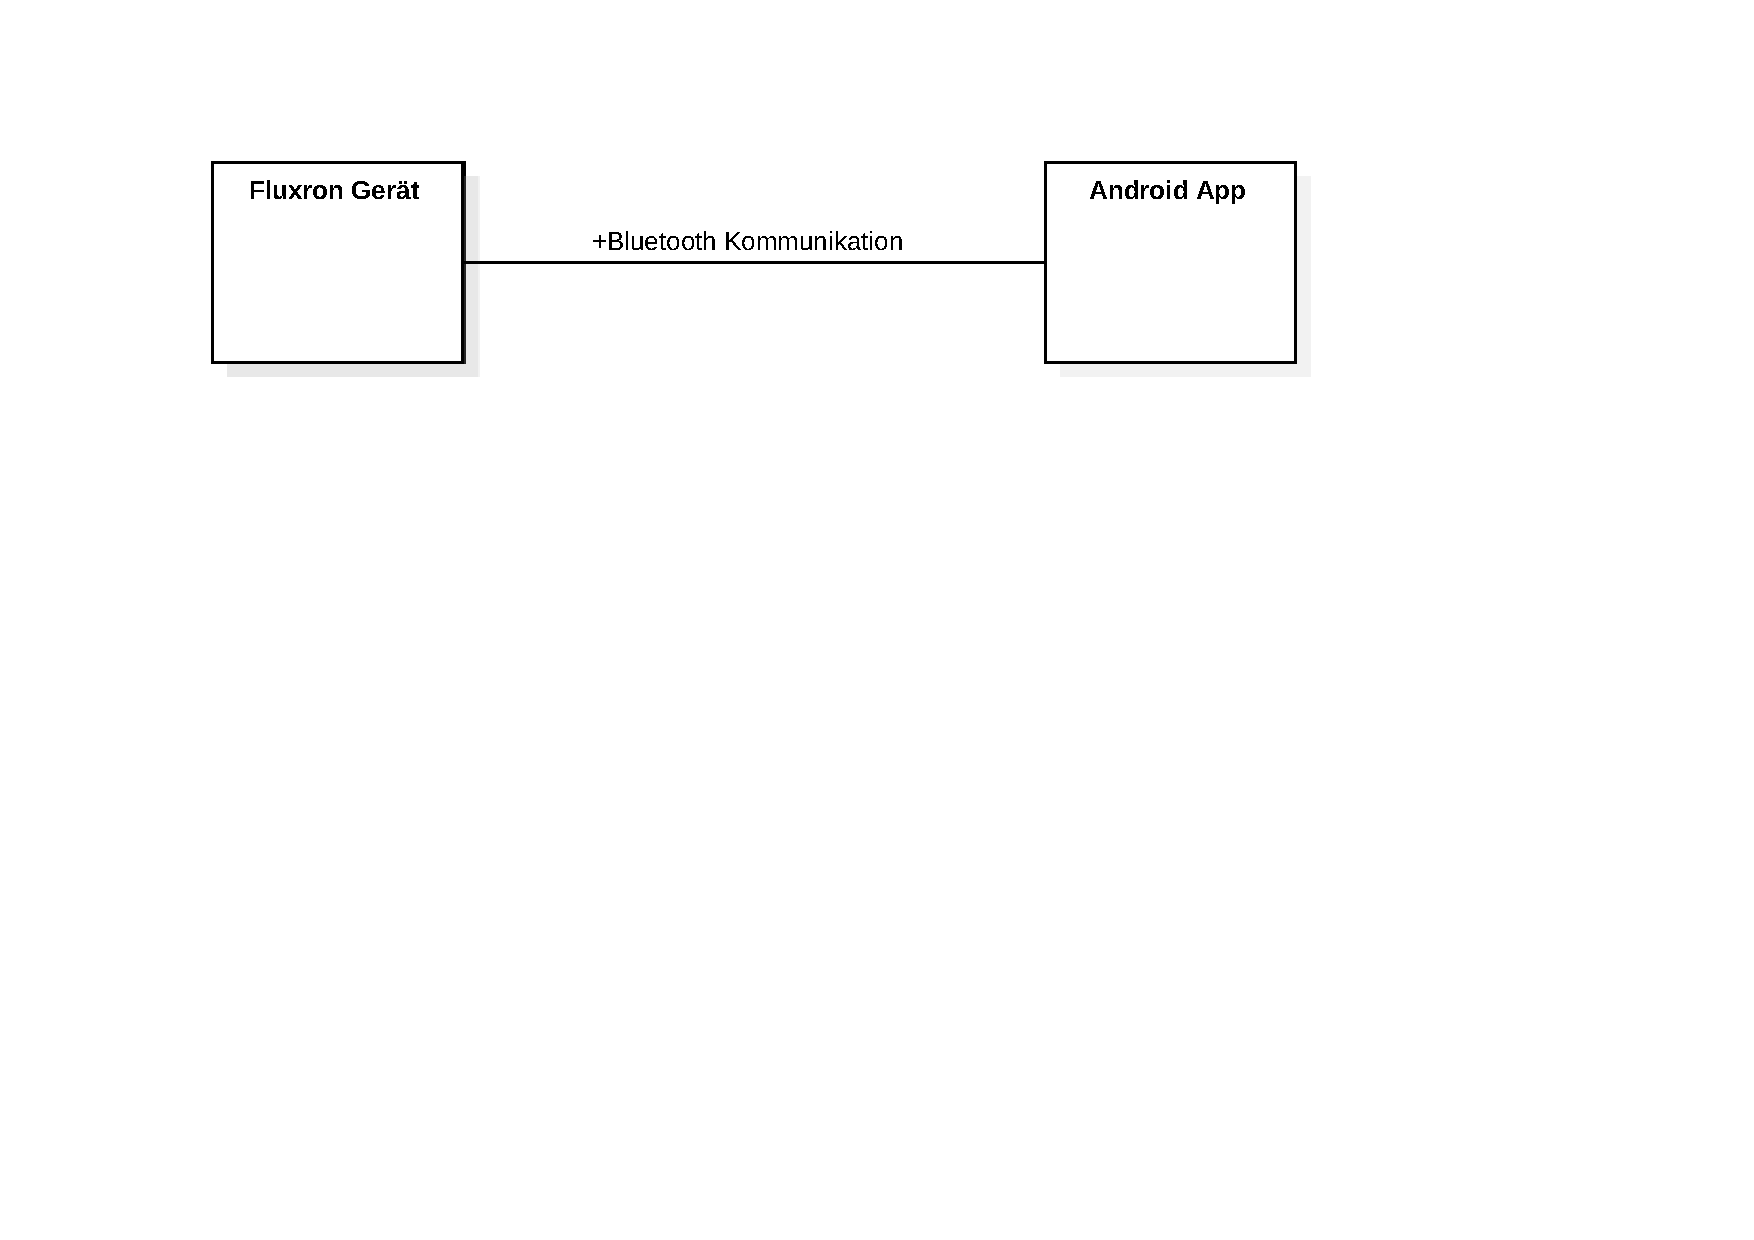
\includegraphics[trim=30 420 140 60,clip,width=\textwidth]{design/res/blackbox}
    \end{center}
    \caption{Blackbox Darstellung}
\end{figure}

Die Applikation kommuniziert mit bis zu 150 Fluxron Geräten via Bluetooth. Aufgrund der Natur von Bluetooth Geräten ist mit einer stark asynchronen Kommunikation zu rechnen. Die Architektur der Fluxron Geräte ist bereits vorgegeben. Die Kommunikation  zwischen den Geräten und der Applikation basiert auf CANopen.

Es soll eine Weiterentwicklung der Applikation durch die \fluxron{} möglich sein.

Die konzeptionellen Anforderungen der \ac{FR}15-18 sowie \ac{NFR}2, 3 sollen durch die Architektur unterstützt werden.

\subsection{Variante A: Schichtenarchitektur}
\begin{figure}[H]
    \begin{center}
    		% GFX Trim left bottom right top
        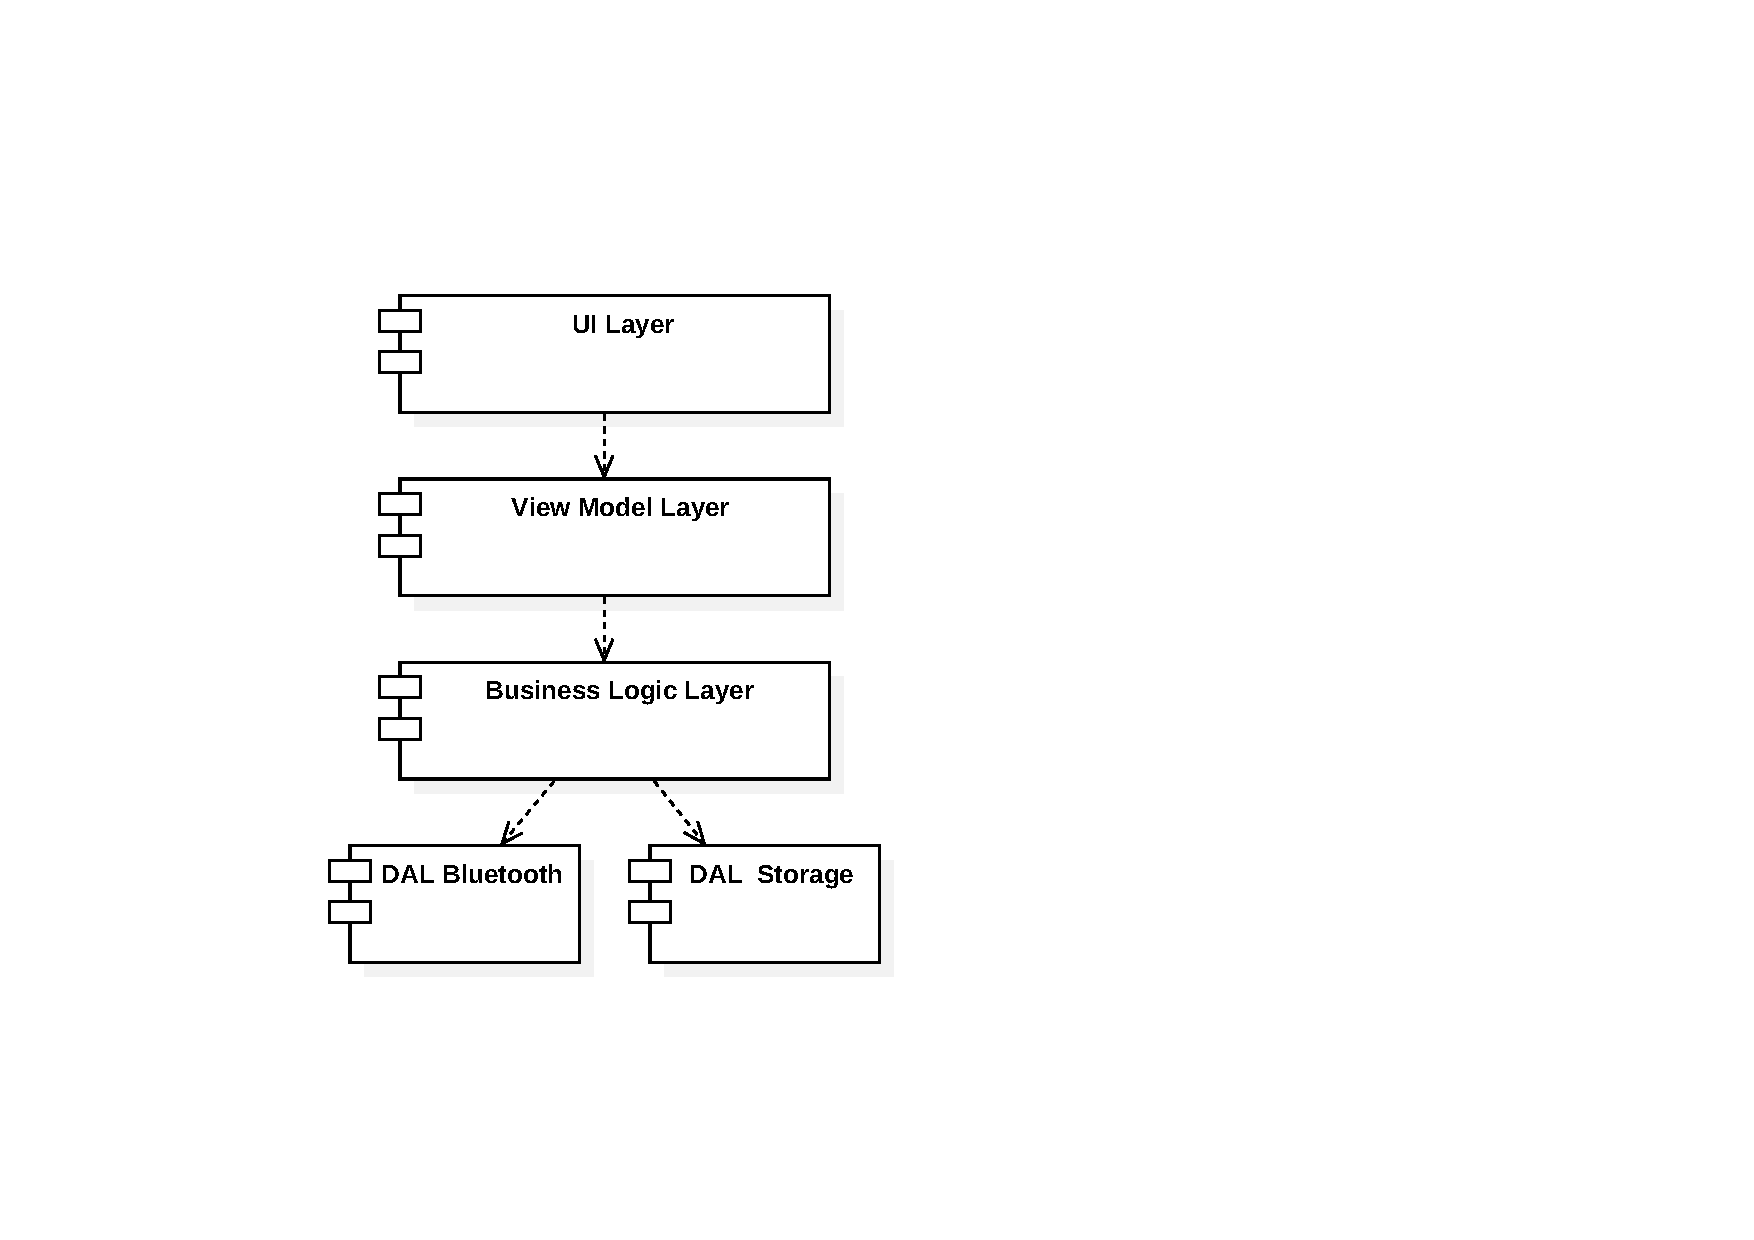
\includegraphics[trim=-100 130 140 110,clip,width=\textwidth]{design/res/layers}
    \end{center}
    \caption{Layer Architektur}
\end{figure}

Die Architektur wird in mehrere Schichten unterteilt. Dabei wird die Kopplung in die Gegenrichtung durch Interfaces und Observer aufgelöst.

\subsection{Variante B: MVC Architektur}
\begin{figure}[H]
    \begin{center}
    		% GFX Trim left bottom right top
        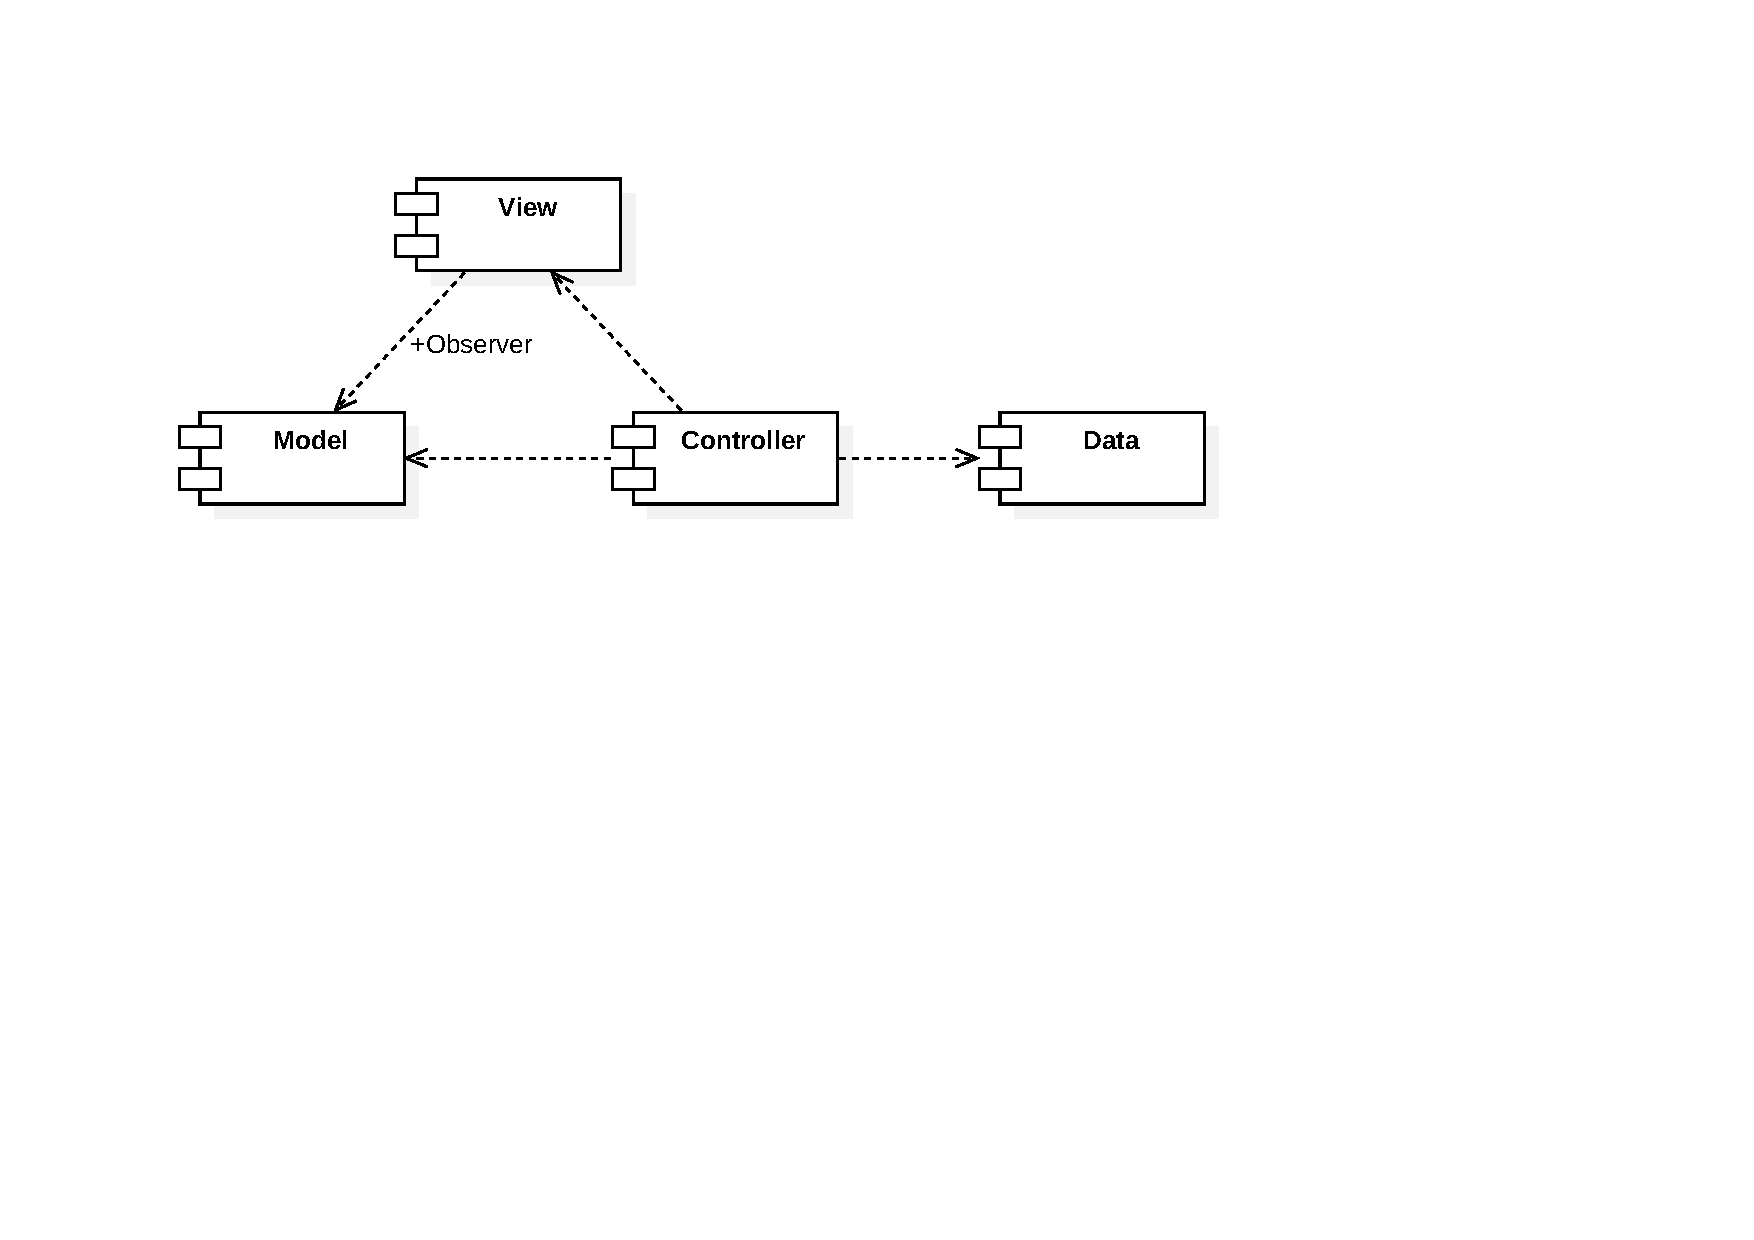
\includegraphics[trim=0 330 140 60,clip,width=\textwidth]{design/res/mvc}
    \end{center}
    \caption{MVC Architektur}
\end{figure}

Weil die Applikation stark durch das User Interface definiert ist, liegt eine Umsetzung mit dem MVC Pattern nahe.

\subsection{Variante C: Event Bus Architektur}
\begin{figure}[H]
    \begin{center}
    		% GFX Trim left bottom right top
        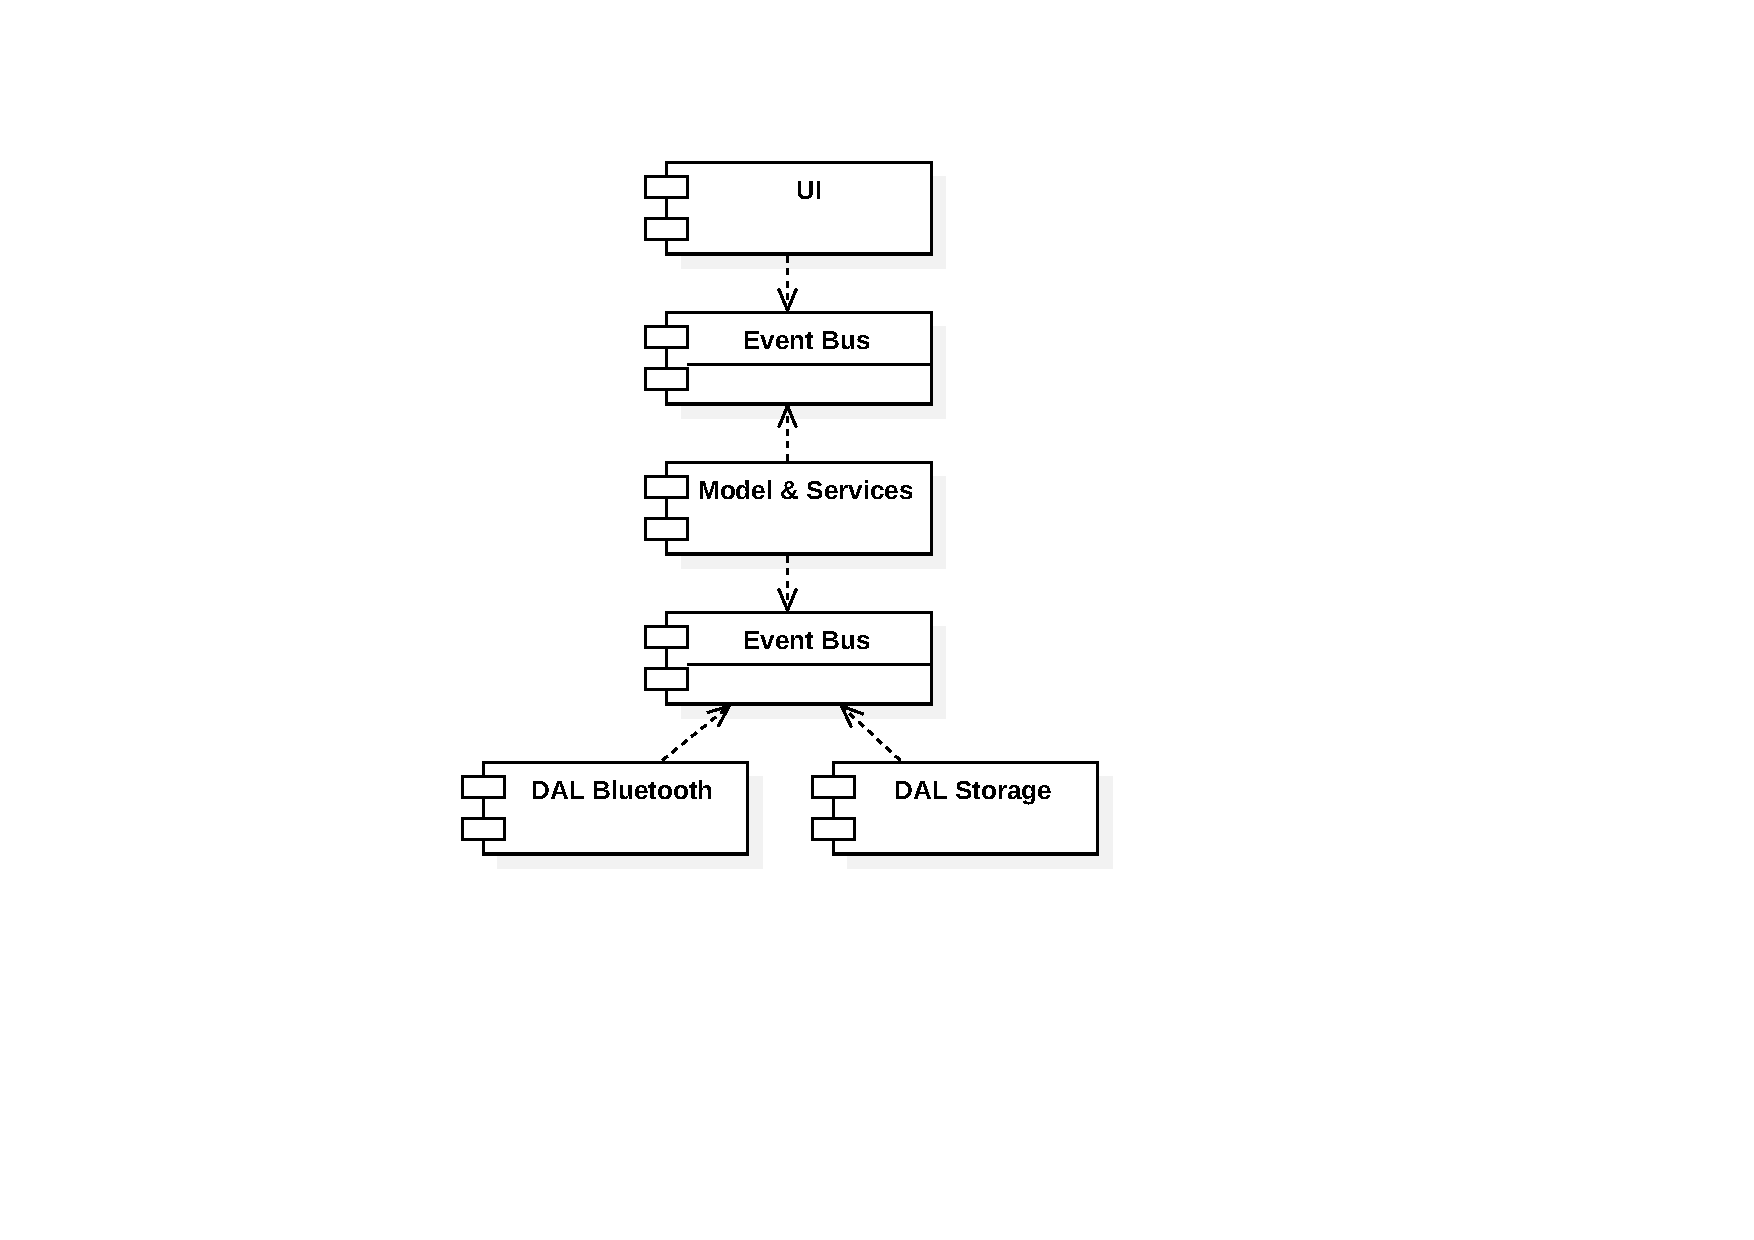
\includegraphics[trim=0 180 100 30,clip,width=\textwidth]{design/res/eventbus}
    \end{center}
    \caption{Event Bus Architektur}
\end{figure}

Mit einem Event Bus zwischen \ac{UI} und Model ist eine stärkere Entkopplung möglich\cite{fowler_event_collab}. Der Event Bus zwischen Model und \ac{DAL} ermöglicht mehrere Module wie Bluetooth und Storage.

\subsection{Bewertung der Architekturmöglichkeiten}

\begin{table}[H]
\begin{tabular}{|p{\textwidth{}/2}|p{\textwidth{}/2}|}
 \hline 
\multicolumn{2}{|c|}{\textbf{Variante A: Schichtenarchitektur}}\\ \hline 
Vorteile
\begin{enumerate}
\item Einfach verständlich, klassische Architektur
\item Separation of Concerns, Low Coupling, High Cohesion
\end{enumerate} & 
Nachteile
\begin{enumerate}
\item \ac{UI} Layer muss ganze Objekthierarchien beobachten
\item Kein einheitliches Parallelitätskonzept
\end{enumerate}
\\ \hline

\multicolumn{2}{|c|}{\textbf{Variante B: MVC Architektur}}\\ \hline 
Vorteile
\begin{enumerate}
\item Gute Entkopplung der View von der Logik
\item Reduktion von Navigationslogik
\end{enumerate} &
Nachteile
\begin{enumerate}
\item \ac{MVC} nur verwendbar in Kombination mit weiteren Patterns
\item Komplexe Observerstruktur zwischen View und Model
\item Kein einheitliches Parallelitätskonzept
\end{enumerate}
\\ \hline

\multicolumn{2}{|c|}{\textbf{Variante C: Event Bus Architektur}}\\ \hline 
Vorteile
\begin{enumerate}
\item Parallelität kann zentral von Bus synchronisiert werden
\item Einfachere und besser gekapselte Komponenten
\item Flache Observerstruktur im User Interface
\item Einfaches Hinzufügen von zusätzlichen Komponenten
\end{enumerate} &
Nachteile
\begin{enumerate}
\item Aufgrund flacher Hierarchie ist es leicht möglich Separation of Concerns zu verletzen.
\item Komplexere Interaktionslogik (Beispiel Message Chains)
\end{enumerate}
\\ \hline
\end{tabular}
\caption{Bewertung Architekturmöglichkeiten}
\end{table}

\subsubsection{Fazit}
Wir entscheiden uns für Variante C, denn sie ermöglicht uns die gewünschte konzeptionelle Erweiterbarkeit in Hinblick auf die \ac{FR} und \ac{NFR} die in Zukunft noch umgesetzt werden sollen. Zudem ermöglicht diese Architektur die Komplexität der Observer stark zu vereinfachen. Die stark asynchrone Kommunikation wird ideal unterstützt.